\documentclass[11pt,a4paper,twoside,pdf]{article}

% Encoding and typography
\usepackage[T1]{fontenc}
\usepackage[utf8]{inputenc}
\usepackage{mathpazo}
\usepackage{braket}

% Mathematics
\usepackage{amsmath, amssymb, amsfonts}
\usepackage{bm}
\usepackage[mathscr]{euscript}

% Figures
\usepackage{graphicx}
\graphicspath{{../figures/}}
\usepackage{float}
\usepackage{subcaption}

% Tables and utilities
\usepackage{multirow}
\usepackage{rotating}
\usepackage{array}
\usepackage{booktabs}
\usepackage{xspace}

% Additional symbols
\usepackage{eurosym}
\usepackage{bbding}
\usepackage{pifont}

% Others
\usepackage{soul}
\usepackage{color}
\usepackage{latexsym}
\usepackage{xtab}

% Hyperlinks
\usepackage[colorlinks=true,urlcolor=blue,linkcolor=blue,citecolor=blue]{hyperref}

% Equation numbering
\numberwithin{equation}{section}

% Margins
\usepackage[top=2.88cm,bottom=2.97cm,left=2.95cm,right=2.95cm]{geometry}

% Language
\usepackage[english]{babel}

% Headers
\usepackage{fancyhdr}

% Theorems
\newtheorem{theorem}{Theorem}[section]
\newtheorem{corollary}{Corollary}[theorem]
\newtheorem{lemma}[theorem]{Lemma}

% Custom commands
\newcommand{\dis}{\displaystyle}

\linespread{1.05}

\begin{document}

% Title page %%%%%%%%%%%%%%%%%%%%%%%%%%%%%%%%%%%%%%%%%%%%%%%%%%%%%%%%%%%%%%%%%%%

\pagestyle{empty}

\noindent
\begin{tabular}{r}

\includegraphics[width=8.8cm]{escudoUGRmonocromo.png} \\[-1.8ex]
\hspace{31mm}\vspace{-8mm}
\begin{tabular}{c}
\hline\\[-1ex]\hskip-2mm
{\bf Facultad de Ciencias}\hspace{18mm}
\end{tabular}
\end{tabular}

\large
\vspace{10mm}
\hspace{25mm}
\begin{tabular}{l}
MASTER'S IN PHYSICS: RADIATION, NANOTECHNOLOGY,\\
PARTICLES AND ASTROPHYSICS

\end{tabular}


\vspace{5mm}
\hspace{25mm}
\begin{tabular}{l}
MATHEMATICAL AND NUMERICAL COMPLEMENTS
\\[1.5ex]
\LARGE\bf SOLVING THE EFIE AND MFIE \\
\LARGE\bf VIA FD-MoM
\end{tabular}
%

\hspace{25mm}
\begin{tabular}{l}
By:
\\
{\bf A. S. Amari Rabah}\\


\end{tabular}
%


\begin{abstract}

The application of the Method of Moments to two-dimensional electromagnetic scattering problems in TM polarization is analyzed, employing the EFIE and MFIE formulations for a perfect electric conductor cylinder. The integral equations are discretized using pulse basis functions and point matching, and are solved by exploiting the circulant structure of the impedance matrix. The numerical solutions for the surface current and the radar cross section are compared with analytical solutions, assessing their accuracy through the $L^2$ norm. The results show rapid convergence of the EFIE, while the MFIE exhibits greater sensitivity to the discretization.

\end{abstract}

% Indice %%%%%%%%%%%%%%%%%%%%%%%%%%%%%%%%%%%%%%%%%%%%%%%%%%%%%%%%%%%%%%%%%%%%%%%

\tableofcontents

% Text %%%%%%%%%%%%%%%%%%%%%%%%%%%%%%%%%%%%%%%%%%%%%%%%%%%%%%%%%%%%%%%%%%%%%%%%

\pagestyle{fancy}
\fancyhead[RO,LE]{\leftmark}
\fancyhead[LO,RE]{\thepage}
\fancyfoot{}



\newpage


\section{Introduction}


For the analysis of electromagnetic systems operating with sinusoidal time variations, it is convenient to transform Maxwell's equations from the time domain to the frequency domain. Assuming a time dependence of the form $\mathbf{F}(\mathbf{r}, t) = \mathfrak{R} \left[ \mathbf{F}(\mathbf{r})e^{j\omega t} \right]$, where $\omega$ is the angular frequency ($\omega = 2\pi f$), the time derivative $\frac{\partial}{\partial t}$ is replaced by the factor $j\omega$. Under this convention, the equations for time-harmonic fields in a macroscopic, homogeneous, linear, and isotropic medium are rewritten in their phasor form as \cite{martin2021campo}:

\begin{equation}
\nabla \cdot \tilde{\mathbf{E}} = \frac{\rho}{\epsilon_0}
\label{leyGauss}
\end{equation}

\begin{equation}
\nabla \cdot \tilde{\mathbf{B}} = 0
\end{equation}

\begin{equation}
\nabla \times \tilde{\mathbf{E}} = -j\omega \tilde{\mathbf{B}}
\label{rotE}
\end{equation}

\begin{equation}
\nabla \times \tilde{\mathbf{B}} = \mu_0\tilde{\mathbf{J}} + j\omega\mu_0\epsilon_0 \tilde{\mathbf{E}}
\label{rotH}
\end{equation}


Where $\mathbf{E}$ is the electric field, $\mathbf{B}$ is the magnetic field, $\rho$ denotes the charge density, and $\mathbf{J}$ the current density.

In linear material media, these quantities can be related to the magnetic field intensity $\mathbf{H}$ and the electric displacement vector $\mathbf{D}$ through the constitutive relations $\mathbf{D} = \epsilon \mathbf{E}$ and $\mathbf{B} = \mu \mathbf{H}$, where $\epsilon = \epsilon_r \epsilon_0$ is the dielectric constant and $\mu = \mu_r \mu_0$ the magnetic permeability of the material.


%---------------------------------------------------------




\subsection{Integral equations}


The equations to be solved for computing the fields $\mathbf{E}$ and $\mathbf{H}$ induced by a current density $\mathbf{J(r)}$ supported within a volume $V$ are derived below.\\

Taking the curl of equation \ref{rotE} and substituting from \ref{rotH}, one obtains

\begin{equation}
\nabla \times \nabla \times \mathbf{E} = -j\omega\nabla \times \mathbf{B} = -j\omega\mu(\mathbf{J} + j\omega\epsilon\mathbf{E}).
\notag
\end{equation}

Using the vector identity $\nabla \times \nabla \times \mathbf{E} = \nabla(\nabla \cdot \mathbf{E}) - \nabla^2 \mathbf{E}$ and defining the wavenumber as $k = \omega\sqrt{\mu\epsilon}$, the expression becomes
\begin{equation}
\nabla(\nabla \cdot \mathbf{E}) - \nabla^2 \mathbf{E} - k^2\mathbf{E} = -j\omega\mu\mathbf{J}.
\notag
\end{equation}

Using Gauss's law \ref{leyGauss}, a Helmholtz equation for the electric field is obtained:
\begin{equation}
\nabla^2 \mathbf{E} + k^2 \mathbf{E} = j\omega\mu\mathbf{J} + \frac{1}{\epsilon}\nabla\rho
\notag
\end{equation}

The explicit dependence on the charge $\rho$ can be eliminated by employing the continuity equation $\nabla \cdot \mathbf{J} = -j\omega\rho$, which allows writing the electric field as a function of the current $\mathbf{J}$ alone

\begin{equation}
\nabla^2 \mathbf{E} + k^2 \mathbf{E} = j\omega\mu\mathbf{J} + \frac{1}{j\omega\epsilon}\nabla(\nabla \cdot \mathbf{J}).
\notag
\end{equation}

The general solution of this equation in an unbounded region is obtained by convolution with the scalar Green's function

\begin{equation}
\mathbf{E}(\mathbf{r}) = -j\omega\mu \int_{V'}   \left[  \mathbf{J}(\mathbf{r}') + \frac{1}{k^2} \nabla' (\nabla' \cdot \mathbf{J}(\mathbf{r}'))  \right] G(\mathbf{r}, \mathbf{r}') d\bm{r'}.
\label{Epuro}
\end{equation}



Similarly, for the field $\mathbf{H}$ the Helmholtz equation is obtained

\begin{equation}
\label{eq:helmholtz_H}
\nabla^2 \mathbf{H} + k^2 \mathbf{H}
=
- \nabla \times \mathbf{J}.
\notag
\end{equation}

With solution

\begin{equation}
\mathbf{H}(\mathbf{r})
=
\int_{V}
\left[
\nabla' \times \mathbf{J}(\mathbf{r}')
\right]
G(\mathbf{r},\mathbf{r}')
\, d\bm{r'}.
\label{Hpuro}
\notag
\end{equation}



From this point onward, the analysis in this work focuses on surfaces that are infinite along a symmetry direction denoted by $z$, which implies that the currents $\mathbf{J}$ induced for both fields are surface currents.

In this way, in equation \ref{Hpuro} the operator $(\nabla' \times)$ can be transferred to the Green's function using the identity $ G(\mathbf{r}, \mathbf{r'}) \nabla' \times \mathbf{J(\mathbf{r'})} = -\nabla' \times \left[ \mathbf{J}(\mathbf{r'}) \cdot G(\mathbf{r}, \mathbf{r'}) \right]  + \nabla'G(\mathbf{r}, \mathbf{r'}) \times J(\mathbf{r'})$. By applying Gauss's theorem, the term $\int_{S'}  \mathbf{J}(\mathbf{r'}) G(\mathbf{r}, \mathbf{r'}) \cdot \bm{\hat{n}} dS' $ vanishes since the currents are perpendicular to the surface normal vector. Finally, using the antisymmetry of the cross product


\begin{equation}
\mathbf{H}(\mathbf{r})
=
\int_{V'}
 \mathbf{J}(\mathbf{r}') \times \nabla'
G(\mathbf{r},\mathbf{r}')
\, d\bm{r'}.
\label{Hpuro2}
\end{equation}



Furthermore, the \textit{effective} Green's function becomes:

\[
G(\bm{\rho}, \bm{\rho'}) = \int_{-\infty}^{+\infty} G(\mathbf{r}, \mathbf{r'}) dz' = \int_{-\infty}^{+\infty} \frac{e^{-jk\sqrt{(|\bm{\rho} - \bm{\rho'}|)^2 + z'^2 }}}{ 4\pi \sqrt{(|\bm{\rho} - \bm{\rho'}|)^2 + z'^2 } } dz' = -\frac{j}{4} H^{(2)}_0(k|\bm{\rho} - \bm{\rho'}| )
\]

Where $H^{(2)}_0(x)$ is the Hankel function of the second kind of order zero.\\




Using the continuity conditions on the electromagnetic fields, relations between the incident and scattered fields in scattering problems can be obtained.

Considering a conducting surface $S$ with outward unit normal vector $\mathbf{\hat{n}}(\mathbf{r})$, the continuity conditions on the tangential components of the fields are:

\begin{equation}
    \mathbf{\hat{n}} \times (\mathbf{E}_{ext} - \mathbf{E}_{int}) = 0, \qquad \mathbf{\hat{n}} \times (\mathbf{H}_{ext} - \mathbf{H}_{int}) = \mathbf{J_s}.
\end{equation}

Where $\mathbf{J_s}$ is the surface current. Restricting to perfect electric conductor ($PEC$) surfaces where the interior fields vanish, and decomposing the exterior fields into incident ($i$) and scattered ($s$) components, the conditions become \cite{martin2021campo}

\begin{equation}
    \mathbf{\hat{n}} \times (\mathbf{E}^{i} + \mathbf{E}^{s}) = 0, \qquad \mathbf{\hat{n}} \times (\mathbf{H}^{i} + \mathbf{H}^{s}) = \mathbf{J_s}.
\end{equation}


Where the incident field is considered known and the scattered field is that created by the currents induced by the incident field on the surface $S$, i.e., the scattered field obeys equations \ref{Epuro} and \ref{Hpuro}.

In this way, the Electric Field Integral Equation (EFIE) is obtained



\begin{equation}
\mathbf{\hat{n}(\mathbf{r})} \times \mathbf{E}^i(\mathbf{r}) = \mathbf{\hat{n} (\mathbf{r})} \times \left( j\omega\mu \int_S \left[ \mathbf{J}(\mathbf{r}') + \frac{1}{k^2} \nabla' (\nabla' \cdot \mathbf{J}(\mathbf{r}')) \right] G(\mathbf{r}, \mathbf{r}') d\mathbf{r'} \right).
\label{EFIE}
\end{equation}


The derivation of the Magnetic Field Integral Equation (MFIE) involves a subtlety regarding the jump due to the current $\bm{J_s}$ that is not present in the EFIE, since the tangential electric field is continuous.

When evaluating the integral \ref{Hpuro2} at points $\bm{r} \to \bm{r'}$, the gradient of the Green's function exhibits a singular behavior of the form $\nabla'G(\mathbf{r}, \mathbf{r}') \sim \frac{\bm{\hat{R}}}{\bm{R}^2}$. Intuitively, one considers an infinitesimal sphere around the singular point where only the half exterior to the PEC contributes to the scattered field, which gives rise to a factor of $1/2$ in the current \cite{gibson2021method}. Thus, the MFIE takes the form




\begin{equation}
\bm{\mathbf{\hat{n}}}(\bm{r}) \times \mathbf{H^i}(\mathbf{r})
= \frac{\bm{J(\mathbf{r})}}{2} - \mathbf{\hat{n}} (\mathbf{r}) \times  \int_{S}
 \mathbf{J}(\mathbf{r}') \times \nabla'
G(\mathbf{r},\mathbf{r}')
\, d\bm{r'}.
\label{MFIE}
\end{equation}\\



\subsubsection{Far field}



When the observation point is located far from the source ($kr \gg 1$), approximations can be made that considerably simplify the computation of the radiated field. In this case, the vectors $\mathbf{r}$ and $\mathbf{r}-\mathbf{r}'$ are nearly parallel; under this assumption, $r$ can be approximated as \cite{martin2021campo}

\begin{equation}
r \approx
\begin{cases}
r - \mathbf{r}' \cdot \hat{\mathbf{r}}, & \text{for phase variations}, \\
r, & \text{for amplitude variations}.
\end{cases}
\label{eq:farfield_r}
\end{equation}

In equation \ref{Epuro}, the differential operators $\nabla'$ and $\nabla' \cdot$ introduce an overall $1/r^2$ dependence, so that neglecting this term in the current, in two dimensions, the far-field radiated electric field is given by

\begin{equation}
\mathbf{E}(\boldsymbol{\rho})
=
- \frac{\omega \mu}{4}
\int
\mathbf{J}(\boldsymbol{\rho}')
H_0^{(2)}\left(k|\boldsymbol{\rho}-\boldsymbol{\rho}'|\right)
\, d\boldsymbol{\rho}'.
\label{eq:farfield_2D}
\end{equation}

And using the large-argument approximation of the Hankel function

\begin{equation}
H_n^{(2)}(k\rho)
\approx
\sqrt{\frac{2j}{\pi k\rho}}
\, j^n e^{-jk\rho},
\quad \rho \rightarrow \infty,
\notag
\end{equation}

the far-field electric field is expressed as

\begin{equation}
\mathbf{E}(\boldsymbol{\rho})
=
- \omega \mu
\sqrt{\frac{j}{8\pi k}}
\frac{e^{-jk\rho}}{\sqrt{\rho}}
\int
\mathbf{J}(\boldsymbol{\rho}')
e^{jk \boldsymbol{\rho}' \cdot \hat{\boldsymbol{\rho}}}
\, d\boldsymbol{\rho}'.
\label{Elejano}
\end{equation}

In two-dimensional scattering problems, the radar cross section $\sigma_{2D}$ is defined as

\begin{equation}
\sigma_{2D}
= \lim_{\rho \to \infty}
2\pi \rho
\frac{|\mathbf{E}^s|^2}{|\mathbf{E}^i|^2}.
\notag
\end{equation}

For computational evaluation, $|\mathbf{E}^i| = 1$ is taken and the far-field distance $\boldsymbol{\rho}$ is set equal to $10^3$ times the characteristic dimension of the object (the radius in the case of the cylinder).








\subsubsection{Combined Field and Physical Optics approximation}

When applied to closed surfaces, the EFIE and MFIE formulations do not guarantee
a unique solution for all frequencies \cite{gibson2021method}. This is due to the existence of
homogeneous solutions that satisfy the boundary conditions in the absence of an incident field.
These spurious solutions correspond to internal resonant modes of the object,
which do not radiate energy to the exterior. The fundamental
cause of this problem lies in the fact that the tangential components of a single
incident field are not sufficient to uniquely determine the surface
current at these frequencies.


The most widely used method to eliminate the internal resonance problem is the
Combined Field Integral Equation (CFIE)
\begin{equation}
\mathrm{CFIE} = \alpha\, \mathrm{EFIE} + (1-\alpha)\, \mathrm{MFIE},
\end{equation}
where $0.5 \leq \alpha \leq 1$ is chosen so as to eliminate the spurious solutions.

The CFIE does not produce physically uncorrelated responses because the resonances of the EFIE and
the MFIE occur at different frequencies, which guarantees the uniqueness of the solution over the entire range. Furthermore, this formulation does not require the introduction of auxiliary
surfaces and maintains the same number of unknowns as the EFIE and MFIE separately.\\


Finally, in the high-frequency regime, the integral term involving the Green's function in expression \ref{MFIE} can be neglected because its rapid phase oscillation causes the total contribution to the integral to be nearly zero. This yields the Physical Optics (PO) approximation: $\boldsymbol{J}(\boldsymbol{r})_{PO} = 2 \boldsymbol{\hat{n}}(\boldsymbol{r}) \times \boldsymbol{H^i} (\boldsymbol{r})
$.







%------------------------------------------------------------------





\subsection{The Method of Moments}



Solving equations \ref{EFIE} and \ref{MFIE} is extremely complex if the system does not possess some form of symmetry that simplifies the integrals. Below, the Method of Moments (MoM) is introduced, which transforms the integro-differential problem into an algebraic one \cite{harrington1993field}.\\

The general MoM formulation is applied to a problem of the form

\begin{equation}
    \mathscr{L} (I) = V.
\label{MoM}
\end{equation}



Where $\mathscr{L}$ is a linear operator, $V$ is called the \textit{system excitation}, and $I$ is the unknown (\textit{system response function}). The unknown $I$ is expanded in $N$ known \textit{basis} functions that are expected to be able to replicate the unknown

$$
    I = \sum_{n=1}^N i_n b_n.
$$

The inner product or \textit{moment} between a basis function $b_n$ and a \textit{weighting} function $p_m$ is defined as

$$
   \braket{p_m, b_n} = \int_{p_m} p_m({\mathbf{r}}) \int_{b_n} b_n({\mathbf{r'}}) d\mathbf{r'} d\mathbf{r}.
$$

Taking the product of $N$ weighting functions $p_m$ with equation \ref{MoM} yields

$$
    \sum_{n=1}^N i_n \braket{p_m, \mathscr{L}(b_n)} = \braket{p_m, V}
$$

Which can be expressed as a matrix system by introducing the \textit{impedance} matrix $Z$

$$
    Z_{mn} = \braket{p_m, \mathscr{L}(b_n)},
$$

obtaining the system of equations

\begin{equation}
    Z \mathbf{I} = \mathbf{V}.
\label{ZIV}
\end{equation}

Where the vector $\mathbf{I}$ contains the unknown coefficients $i_n$ and the vector $\mathbf{V}$ the products $\braket{p_m, V}$.

The basis functions are chosen so that the integral equations are evaluated at a discrete set of points, which mathematically corresponds to taking Dirac delta weighting functions ($p_m(\mathbf{r}) = \delta(\mathbf{r})$). Although this method (called \textit{point matching}) has the advantage of eliminating one integral when evaluating the terms of $Z$, it also has the disadvantage of imposing the incident field conditions only at specific points.


Similarly, \textit{pulse} functions are used as basis functions. The domain is divided into $N$ equally spaced points, and the pulse function is defined as

$$
    b_n(x) =
    \begin{cases}
        1 \quad \text{if}  \quad x_n \leq x \leq x_{n+1}, \\
        0  \quad  \text{else}.
    \end{cases}
$$

Pulse functions represent a crude approximation of the solution, but they greatly facilitate the evaluation of the integrals. Indeed, if the spatial discretization is sufficiently fine, the centroid approximation can be used to evaluate the integrals in the terms of $Z_{mn}$.

Pulse functions impose an even greater restriction in the treatment of operators, especially those involving derivatives. For instance, in the EFIE \ref{EFIE}, the term $\nabla' \cdot \mathbf{J(\mathbf{r'})}$ would not be well defined when decomposing the current into functions of this type. For this reason, functions with a well-defined divergence (such as triangular or RWG-type functions) are more appropriate in these cases.
In the following section, this issue is resolved by restricting the polarization of the incident field to only the perpendicular (TM) one.










\section{Integral equations in TM polarization}



A plane wave with incidence angle $\phi^i$ in TM polarization is considered, with electric field:

\begin{equation}
\mathbf{E}^i(\boldsymbol{\rho}) = e^{j k \hat{\boldsymbol{\rho}}_i \cdot \boldsymbol{\rho}} \, \hat{\mathbf{z}}
= e^{j k (x \cos \phi^i + y \sin \phi^i)} \, \hat{\mathbf{z}},
\label{ondaplanaincidente}
\end{equation}

and corresponding magnetic field

\begin{equation}
\mathbf{H}^i(\boldsymbol{\rho})
= - \hat{\boldsymbol{\rho}}_i \times \frac{\mathbf{E}^i}{\eta}
= \frac{1}{\eta}
\left(
- \sin \phi^i \, \hat{\mathbf{x}}
+ \cos \phi^i \, \hat{\mathbf{y}}
\right)
e^{j k (x \cos \phi^i + y \sin \phi^i)},
\label{ondaplanaH}
\end{equation}

where $\eta = \sqrt{\mu/\varepsilon}$ and
$\hat{\boldsymbol{\rho}}_i = \cos \phi^i \, \hat{\mathbf{x}} + \sin \phi^i \, \hat{\mathbf{y}}$.
Since the incident field has only a component in the $\hat{\mathbf{z}}$ direction, the induced surface current density $\mathbf{J}$ also has a component only in $\hat{\mathbf{z}}$.

\subsection{EFIE in TM polarization}

The EFIE \ref{EFIE} simplifies to

\begin{equation}
E_z^i(\bm{\rho})
= j \omega \mu
\int_C
G(\boldsymbol{\rho}, \boldsymbol{\rho}')
\left[
J_z(\boldsymbol{\rho}')
+ \frac{1}{k^2} \nabla' \nabla' \cdot J_z(\boldsymbol{\rho'})
\right]
\, d\boldsymbol{\rho'}
\label{ondaplana}
\end{equation}

where $C$ is an arbitrary two-dimensional contour.

Since $\boldsymbol{J}$ has only a component in $\boldsymbol{\hat{z}}$, the problematic divergence term vanishes because the current is symmetric in $z$. Substituting the Green's function yields


\begin{equation}
\frac{4}{\omega \mu}
E_z^i(\boldsymbol{\rho})
=
\int_C
J_z(\boldsymbol{\rho}')
\, H_0^{(2)}\!\left( k \lvert \boldsymbol{\rho} - \boldsymbol{\rho}' \rvert \right)
\, d\boldsymbol{\rho}'
\end{equation}




Applying basis and weighting functions $b_n$ and $p_m$ respectively, the impedance matrix is

\begin{equation}
Z^{EFIE}_{mn}
=
\int_{p_m}
p_m(\boldsymbol{\rho})
\int_{b_n}
b_n(\boldsymbol{\rho}')
\, H_0^{(2)}\!\left( k \lvert \boldsymbol{\rho} - \boldsymbol{\rho}' \rvert \right)
\, d\boldsymbol{\rho}'
\, d\boldsymbol{\rho},
\label{ZEFIE}
\end{equation}

and excitation vector

\begin{equation}
V^{EFIE}_m
=
\frac{4}{\omega \mu}
\int_{p_m}
p_m(\boldsymbol{\rho})
\, E_z^i(\boldsymbol{\rho})
\, d\boldsymbol{\rho}
\label{VmEFIE}
\end{equation}

\subsection{MFIE in TM polarization}

Similarly for the MFIE, since the current has only a $\boldsymbol{\hat{z}}$ component, the only portion of the incident field that contributes to the current is the one tangent to $C$. Therefore, equation \ref{MFIE} becomes

\begin{equation}
\hat{\mathbf{t}}(\boldsymbol{\rho}) \cdot \mathbf{H}^i(\boldsymbol{\rho})
=
\frac{J_z(\boldsymbol{\rho})}{2}
-
\frac{j}{4}
\hat{\mathbf{z}} \cdot
\left[
\hat{\mathbf{n}}(\boldsymbol{\rho}) \times
\int_{C}
J_z(\boldsymbol{\rho}')
\hat{\mathbf{z}} \times
\nabla' H_0^{(2)}\!\left( k \lvert \boldsymbol{\rho} - \boldsymbol{\rho}' \rvert \right)
\, d\boldsymbol{\rho}'
\right],
\label{MFIEtan}
\end{equation}

where the tangent vector is
$\hat{\mathbf{t}}(\boldsymbol{\rho}) = \hat{\mathbf{n}}(\boldsymbol{\rho}) \times \hat{\mathbf{z}}$.
Applying the vector identity $\mathbf{A} \times \mathbf{B} \times \mathbf{C}
=
(\mathbf{A} \cdot \mathbf{C}) \mathbf{B}
-
(\mathbf{A} \cdot \mathbf{B}) \mathbf{C}$

\begin{equation}
\hat{\mathbf{n}}(\boldsymbol{\rho}) \times
\hat{\mathbf{z}} \times
\nabla H_0^{(2)}\!\left( k \lvert \boldsymbol{\rho} - \boldsymbol{\rho}' \rvert \right)
=
\hat{\mathbf{z}}
\left[
\hat{\mathbf{n}}(\boldsymbol{\rho}) \cdot
\nabla' H_0^{(2)}\!\left( k \lvert \boldsymbol{\rho} - \boldsymbol{\rho}' \rvert \right)
\right],
\end{equation}

since
$\hat{\mathbf{n}} \cdot \hat{\mathbf{z}} = 0$
along the entire contour $C$.
Substituting this into \ref{MFIEtan} yields

\begin{equation}
\hat{\mathbf{t}}(\boldsymbol{\rho}) \cdot \mathbf{H}^i(\boldsymbol{\rho})
=
\frac{J_z(\boldsymbol{\rho})}{2}
-
\frac{j}{4}
\int_{C}
J_z(\boldsymbol{\rho}')
\left[
\hat{\mathbf{n}}(\boldsymbol{\rho}) \cdot
\nabla' H_0^{(2)}\!\left( k \lvert \boldsymbol{\rho} - \boldsymbol{\rho}' \rvert \right)
\right]
\, d\boldsymbol{\rho'}.
\end{equation}

Furthermore, since

\begin{equation}
\nabla' H_0^{(2)}\!\left( k \lvert \boldsymbol{\rho} - \boldsymbol{\rho}' \rvert \right)
=
- k H_1^{(2)}\!\left( k \lvert \boldsymbol{\rho} - \boldsymbol{\rho}' \rvert \right)
\left[
\frac{x - x'}{R} \hat{\mathbf{x}}
+
\frac{y - y'}{R} \hat{\mathbf{y}}
\right],
\end{equation}

the two-dimensional MFIE for TM polarization can be written as

\begin{equation}
\hat{\mathbf{t}}(\boldsymbol{\rho}) \cdot \mathbf{H}^i(\boldsymbol{\rho})
=
\frac{J_z(\boldsymbol{\rho})}{2}
+
\frac{j k}{4}
\int_{C'}
\left[
\hat{\mathbf{n}}(\boldsymbol{\rho}) \cdot \hat{\mathbf{R}}
\right]
J_z(\boldsymbol{\rho}')
H_1^{(2)}\!\left( k \lvert \boldsymbol{\rho} - \boldsymbol{\rho}' \rvert \right)
\, d\boldsymbol{\rho}',
\end{equation}

where

\begin{equation}
\hat{\mathbf{R}}
=
\frac{x - x'}{R} \hat{\mathbf{x}}
+
\frac{y - y'}{R} \hat{\mathbf{y}}
=
\frac{\boldsymbol{\rho} - \boldsymbol{\rho}'}{|\boldsymbol{\rho} - \boldsymbol{\rho}'|}.
\end{equation}


Applying basis and weighting functions $b_n$ and $p_m$ respectively, the impedance matrix is:

\begin{equation}
    Z^{MFIE}_{mn}
=
\frac{1}{2}
\int_{p_m \cup b_n}
p_m(\boldsymbol{\rho}) b_n(\boldsymbol{\rho}) \, d\boldsymbol{\rho}
\notag
\end{equation}
\begin{equation}
+
\frac{j k}{4}
\int_{f_m}
p_m(\boldsymbol{\rho})
\int_{b_n}
b_n(\boldsymbol{\rho}')
\left[
\hat{\mathbf{n}}(\boldsymbol{\rho}) \cdot \hat{\mathbf{R}}
\right]
H_1^{(2)}\!\left( k \lvert \boldsymbol{\rho} - \boldsymbol{\rho}' \rvert \right)
\, d\boldsymbol{\rho}'
\, d\boldsymbol{\rho},
\label{ZMFIE}
\end{equation}


where the first integration is carried out over the portions of the contour where $p_m$ and $b_n$ overlap, and the second where they do not.
The elements of the excitation vector are given by

\begin{equation}
V^{MFIE}_m
=
\int_{p_m}
p_m(\boldsymbol{\rho})
\left[
\hat{\mathbf{t}}(\boldsymbol{\rho}) \cdot \mathbf{H}^i(\boldsymbol{\rho})
\right]
\, d\boldsymbol{\rho}.
\end{equation}




\section{Scattering from an infinite cylinder in TM polarization}



The induced currents and scattered field of a two-dimensional cylinder of radius $a$, illuminated by the incident plane wave \ref{ondaplana}, are solved. The exact solution for the induced current $J_z(\phi)$ is \cite{ruck1970radar}:

\begin{equation}
J_z(\phi)
=
\frac{2}{\pi k a \eta}
\sum_{n=0}^{\infty}
\epsilon_n (-j)^n
\frac{\cos n\phi}{H_n^{(1)}(k a)}
\label{Jexacta}
\end{equation}

and the far-field scattered field for an azimuthal incidence angle $\phi^i = 0$ and an observation angle $\phi^s$ is:

\begin{equation}
E^s(\rho, \phi^s)
=
-
\sqrt{\frac{2}{\pi}}
\frac{e^{-j (k \rho - \pi/4)}}{\sqrt{k \rho}}
\sum_{n=0}^{\infty}
\epsilon_n (-1)^n
\cos n\phi^s
\frac{J_n(k a)}{H_n^{(2)}(k a)}
\label{Eexacto}
\end{equation}

where $\epsilon_n = 1$ for $n = 0$, and $\epsilon_n = 2$ otherwise; the series is truncated at $n = 40$ modes in both cases.

For the numerical simulation using the Method of Moments, the cylinder contour is divided into $N$ segments of length $\Delta l = 2\pi a / N$. Point matching centered on the segment and pulse functions are used, yielding $N$ unknowns.


\subsection{MoM EFIE}
\label{efienum}

For terms with $m \neq n$, the centroid approximation is used to evaluate the integral in the impedance matrix \ref{ZEFIE}

$$
    Z^{EFIE}_{mn} =  H_0^{(2)}\!\left( k \lvert \boldsymbol{\rho_m} - \boldsymbol{\rho_n}' \rvert \right) \Delta l.
$$

While the self-terms $n=m$ present a singularity, so using the small-argument approximation of the Hankel function:

\begin{equation}
H_0^{(2)}(k x)
\approx
1
-
j \frac{2}{\pi}
\log\!\left( \frac{\gamma k x}{2} \right),
\qquad x \to 0;
\end{equation}

where $\gamma = e^{\gamma'}$, with $\gamma'$ being the Euler-Mascheroni constant. Therefore, the integral becomes

\begin{equation}
I
=
\int_0^{\Delta l}
\left[
1
-
j \frac{2}{\pi}
\log\!\left(
\frac{\gamma |\boldsymbol{\rho} - \boldsymbol{\rho'}|}{2}
\right)
\right]
d\rho'.
\end{equation}

The logarithmic part of this integral presents a singularity; upon careful integration one obtains

\begin{equation}
I
=
\Delta l
-
j \frac{2}{\pi}
\left[
\Delta l
\log\!\left(
\frac{\gamma k (\Delta l - \rho)}{2 e}
\right)
+
\rho
\log\!\left(
\frac{\rho}{\Delta l - \rho}
\right)
\right],
\end{equation}

and evaluating the outer integral at $\rho = \Delta l / 2$ via point matching, the self-terms $Z_{mm}$ become

\begin{equation}
Z^{EFIE}_{mm}
=
\Delta l
\left[
1
-
j \frac{2}{\pi}
\log\!\left(
\frac{\gamma k \Delta l}{4e}
\right)
\right].
\end{equation}


Finally, the excitation vector \ref{VmEFIE} takes the form

$$
    V^{EFIE}_m = \frac{4}{\omega \mu} e^{jk (x_m cos\phi^i + y_m sin\phi^i)}.
$$



Due to the rotational symmetry of the cylinder and the uniform discretization of the contour into $N$ identical segments, the distance between two centers $m$ and $n$ depends only on their difference $|m-n|$:

$$\lvert \boldsymbol{\rho_m} - \boldsymbol{\rho_n} \rvert = 2a \left| \sin\left( \frac{\pi(m-n)}{N} \right) \right|$$

This implies that the elements of the impedance matrix satisfy the condition $Z_{mn} = Z_{i, (i+(n-m)) \pmod N}$, i.e., $Z$ is a circulant matrix.\newline

This structure allows for a drastic optimization of the computational efficiency in the construction of $Z$. Instead of nesting two \texttt{for} loops over $m$ and $n$ with a cost of $O(N^2)$, only the first row needs to be computed, with a cost of $O(N)$, which also reduces memory usage by computing only one row instead of the entire matrix.

However, it is in solving the system where the greatest efficiency gain is found. In this work, the specialized scientific computing libraries $NumPy$ (ver. \textit{1.26.4}) and $SciPy$ (ver. \textit{1.13.1}) for $Python$ (ver. \textit{3.12.10}) are used \cite{harris2020array, 2020SciPy-NMeth}. Typically, the $NumPy$ function \texttt{linalg.solve()} would be used, which employs an LU factorization with a computational cost of $O(N^3)$. However, by using the $SciPy$ function \texttt{linalg.solve-circulant()} specifically designed for circulant matrices, the system is solved in the spectral domain via the Fast Fourier Transform (FFT), reducing the complexity to $O(N \log N)$.

Finally, once the currents are obtained, the scattered field $\boldsymbol{E^i}$ is computed through equation \ref{Epuro}.\\


\subsubsection{Results}



Figure \ref{fig:resultadosEFIE} shows the numerical results obtained via FD-MoM for the EFIE, together with the analytical solution given by \ref{Eexacto}, for the induced current and the two-dimensional radar cross section of an infinite cylinder of radius $a = 2\lambda$. Different contour discretizations ($\Delta \phi = 2\pi a/ N$) are shown along with the error measured using the $L^2$ norm.

In the case of the induced surface current, for small values of $N$ ($N=10$ and $N=20$) the numerical approximation shows notable deviations from the exact solution. As $N$ increases, the numerical solution gradually converges to the analytical solution, with a notable improvement from $N \geq 40$ onward. For discretizations $N=100$ and $N=1000$, the agreement is nearly complete, with errors on the order of $10^{-4}$. On the other hand, in the representation of the two-dimensional radar cross section, an even faster convergence is observed. For coarse discretizations, spurious oscillations and large errors appear, although these are rapidly attenuated as $N$ increases. From $N \geq 50$ onward, the numerical RCS reproduces the oscillations of the exact solution.





\newpage
\begin{figure}[H]
\centering

\begin{subfigure}{0.95\textwidth}
    \centering
    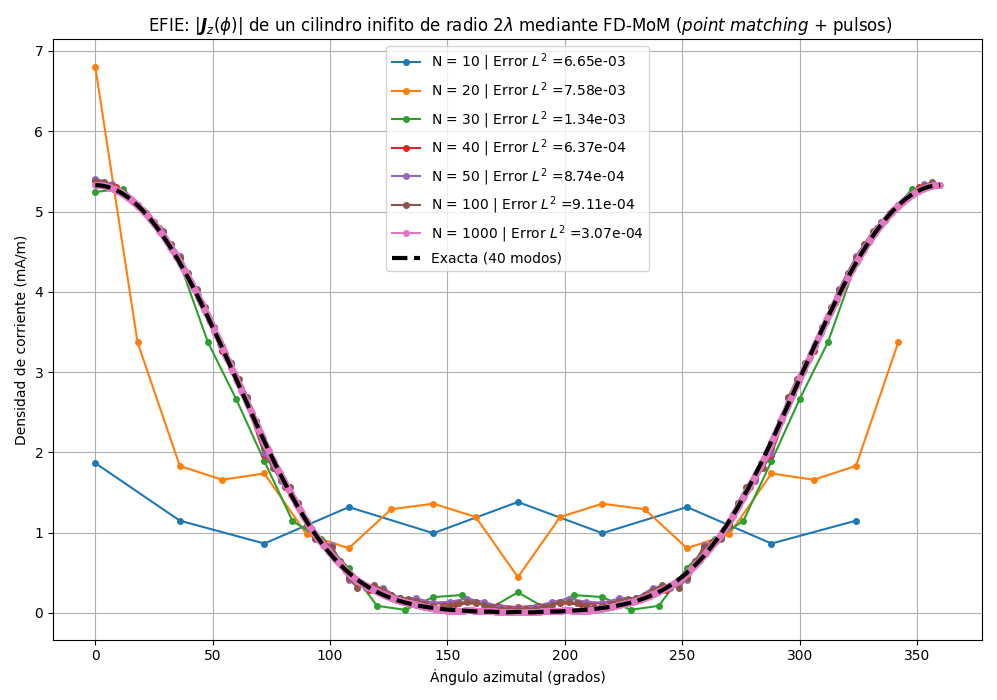
\includegraphics[width=\linewidth]{CorrientesEFIE.png}
    \caption{Magnitude of the induced surface current density $|J_z(\phi)|$ as a function of the azimuthal angle for various values of $N$. The error is taken as the $L^2$ norm of the difference between the analytical solution \ref{Jexacta} and the numerical one described in section \ref{efienum}.}
    \label{fig:corriente}
\end{subfigure}

\vfill

\begin{subfigure}{0.95\textwidth}
    \centering
    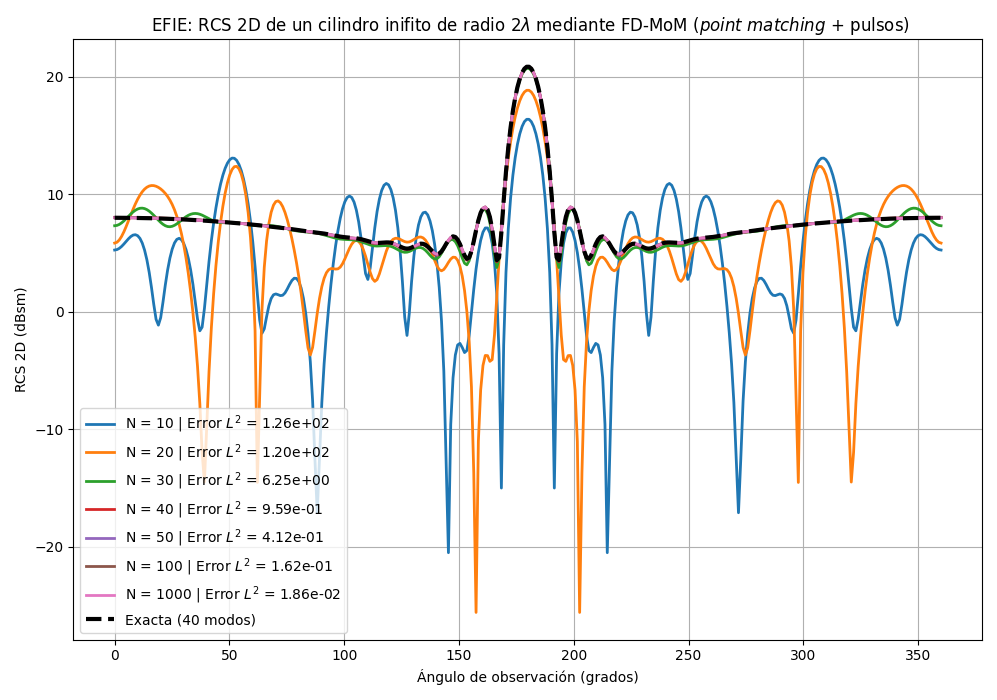
\includegraphics[width=\linewidth]{RCS2DEFIE.png}
    \caption{Two-dimensional radar cross section $\sigma_{2D}(\phi)$ in logarithmic scale (dBsm) as a function of the observation angle for various values of $N$. The error is taken as the $L^2$ norm of the difference between the analytical solution \ref{Eexacto} and the numerical one described in section \ref{efienum}. For the evaluation of $\boldsymbol{E}$ in the far field, expression \ref{Elejano} is used with $\rho = 1000 \cdot 2\lambda$.
    }
    \label{fig:rcs}
\end{subfigure}

\caption{Numerical results obtained via FD-MoM for the EFIE in TM polarization for a PEC conducting cylinder with radius $a = 2\lambda$ illuminated by the incident plane wave \ref{ondaplanaincidente} with $\phi^i=0^\circ$. The angular discretization is $2\pi a/N$. Normalized units in wavelength are used with $\lambda = 1$.}
\label{fig:resultadosEFIE}
\end{figure}










\subsection{MoM MFIE}
\label{mfienum}

In the case of pulse basis functions and point matching, only the first integral of \ref{ZMFIE} contributes to the self-terms

$$
    Z^{MFIE}_{mm} = \frac{1}{2}.
$$

The second integral contributes to the off-diagonal terms; using the centroid approximation

$$
    Z^{MFIE}_{mm} = (\boldsymbol{\hat{n}}_m \cdot \boldsymbol{\hat{R}}_{mn}) \frac{jk\Delta l}{4} H_1^{(2)}\!\left( k \lvert \boldsymbol{\rho}_m - \boldsymbol{\rho}_n \rvert \right)
$$

Where in the case of the cylinder $\boldsymbol{\hat{n}}_m \cdot \boldsymbol{\hat{R}}_{mn} = \frac{\rho_m}{a} \frac{\rho_m - \rho_n}{|\rho_m - \rho_n|}$ and the tangent vector is $\boldsymbol{\hat{t}} (\boldsymbol{\rho}) = sin\phi \boldsymbol{\hat{x}} - cos\phi \boldsymbol{y},$ so the matrix $Z$ is again circulant.\\

Finally, the excitation vector is

$$
    V^{MFIE}_m = -\frac{1}{\eta} (sin\phi_m sin\phi^i + cos\phi_m cos\phi^i) e^{jk (x_m cos\phi^i + y_m sin\phi^i)}.
$$


\subsubsection{Results}




Figure \ref{fig:resultadosMFIE} shows the numerical results obtained via FD-MoM for the MFIE, together with the analytical solution given by \ref{Eexacto}, for the induced current and the two-dimensional radar cross section of an infinite cylinder of radius $a = 2\lambda$. Different contour discretizations ($\Delta \phi = 2\pi a/ N$) are shown along with the error measured using the $L^2$ norm.

In the surface current distribution, it is observed that for small values of $N$ the numerical solution exhibits strong deviations from the exact solution, especially at its extremes. As the number of segments increases, the current gradually converges toward the analytical solution. From $N \geq 40$ onward, the large oscillations disappear, and for discretizations $N = 100$ and $N = 1000$, greater agreement is obtained, with errors on the order of $10^{-4}$.

On the other hand, in the case of the two-dimensional radar cross section, a slower and less regular convergence is observed. For coarse discretizations, large-amplitude spurious oscillations appear along with significant deviations at the minima and maxima. Although these oscillations are reduced as $N$ increases, even for $N = 1000$ small differences persist with respect to the exact solution, with an error on the order of $10^{-1}$.

This can be explained through the nature of the MFIE formulation, which involves derivatives of the Green's function, endowing it with a less regular behavior. The use of pulse basis functions and point matching does not provide a sufficiently smooth representation of the solution. The use of, for example, triangular functions that do have a well-defined divergence would improve the result by capturing the variations in the Green's function.












\newpage
\begin{figure}[H]
\centering

\begin{subfigure}{0.95\textwidth}
    \centering
    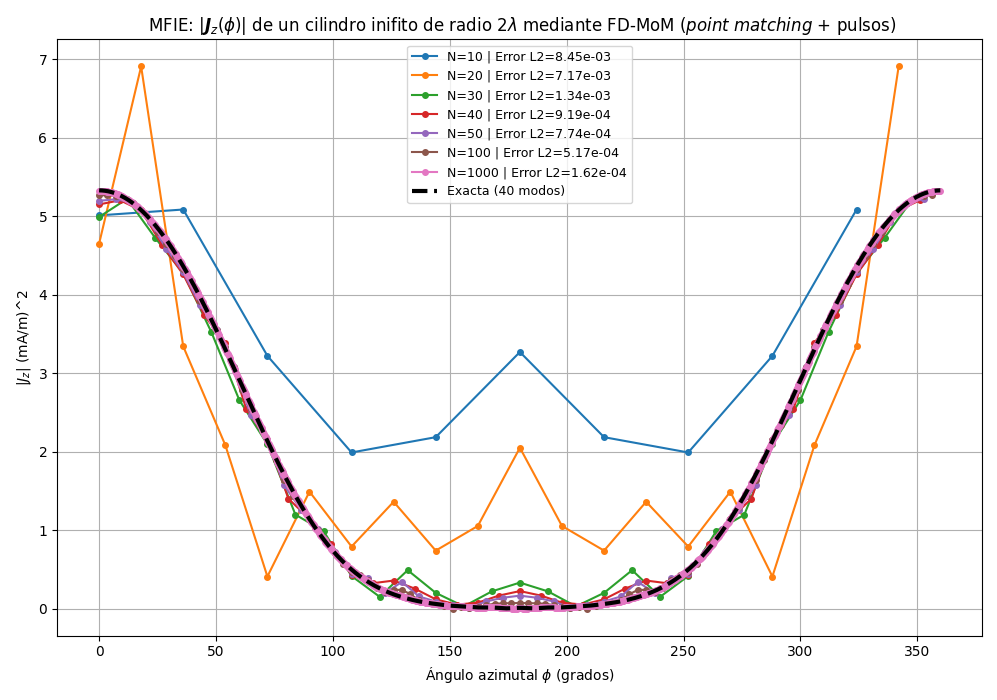
\includegraphics[width=\linewidth]{CorrientesMFIE.png}
    \caption{Magnitude of the induced surface current density $|J_z(\phi)|$ as a function of the azimuthal angle for various values of $N$. The error is taken as the $L^2$ norm of the difference between the analytical solution \ref{Jexacta} and the numerical one described in section \ref{mfienum}.}
    \label{fig:corriente}
\end{subfigure}

\vfill

\begin{subfigure}{0.95\textwidth}
    \centering
    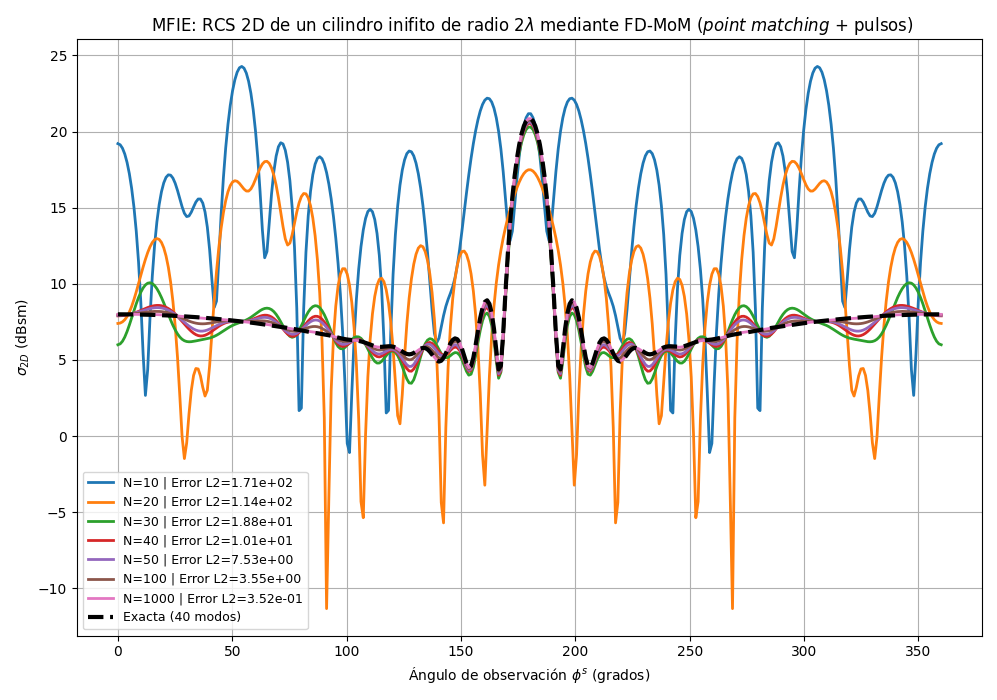
\includegraphics[width=\linewidth]{RCS2DMFIE.png}
    \caption{Two-dimensional radar cross section $\sigma_{2D}(\phi)$ in logarithmic scale (dBsm) as a function of the observation angle for various values of $N$. The error is taken as the $L^2$ norm of the difference between the analytical solution \ref{Eexacto} and the numerical one described in section \ref{mfienum}. Once the currents are obtained through the MFIE, the far-field $E$ is computed using \ref{Elejano} with $\rho = 1000 \cdot 2\lambda$.
    }
    \label{fig:rcs}
\end{subfigure}

\caption{Numerical results obtained via FD-MoM for the MFIE in TM polarization for a PEC conducting cylinder with radius $a = 2\lambda$ illuminated by the incident plane wave \ref{ondaplanaH} with $\phi^i=0^\circ$. The angular discretization is $2\pi a/N$. Normalized units in wavelength are used with $\lambda = 1$.
}
\label{fig:resultadosMFIE}
\end{figure}





\newpage





\section{Conclusion}

In this work, the numerical solution of a two-dimensional electromagnetic scattering problem has been addressed using the Method of Moments, applying it to the EFIE and MFIE formulations for a perfect electric conductor cylinder in TM polarization.

The results obtained show that the EFIE formulation exhibits numerically stable behavior and rapid convergence toward the analytical solution as the number of segments $N$ increases. For sufficiently fine discretizations, the induced surface current and the two-dimensional radar cross section reproduce the exact solution with high accuracy, reaching errors on the order of $10^{-4}$ when pulse basis functions and point matching are employed.

In the case of the MFIE formulation, good convergence is observed for the surface current, similar to that obtained with the EFIE. However, the convergence of the RCS is slower and exhibits greater sensitivity to the discretization. Even for large values of $N$, small discrepancies persist with respect to the analytical solution, reflected in errors larger than those obtained with the EFIE.

This behavior is due to the nature of the MFIE, which involves derivatives of the integral kernel and therefore amplifies the errors associated with insufficiently smooth discretizations. The use of pulse functions and point matching limits the accuracy of the formulation.

The results indicate that the EFIE provides greater overall accuracy, while the MFIE requires more sophisticated discretization schemes to achieve a comparable level of precision. Therefore, for practical applications with simple discretizations, the EFIE constitutes a more suitable choice for two-dimensional electromagnetic scattering analysis.



















\newpage

\bibliographystyle{plain}
\bibliography{bibliografia}





\end{document}
